\section{Algorithms and Datastructures}
\begin{frame}[fragile]
\frametitle{Algorihtms and Datastructures}
\begin{displaymath}
Computer Program = Algorithms + Data Structures
\end{displaymath}
\begin{itemize}
\item Introduction
\item Analysis
\item Algorithmic Toolbox
\item Basic Data Structures
\item Sorting and Searching
\item Trees and Tree Algorithms
\item Graphs and Graph Algorithms
\item String Algorithms
\end{itemize}
\end{frame}

\subsection{Time Measurement}
\begin{frame}[fragile]
\frametitle{Time Measurement}
C++ provides possibilities to measure the time consumption of a given
code fragment. To use these possibilities, the header file \verb|ctime|
must be included.

{\tiny
\begin{lstlisting}
#include <ctime>
#include <iostream>
using namespace std;

int main(int argc, char **argv) {
  clock_t start, stop;
  start = clock();
  
  // CODE FRAGMENT
  
  stop = clock();
  // Time in seconds
  double time = (double)(stop-start)/CLOCKS_PER_SEC;
}
\end{lstlisting}
}
\end{frame}

\begin{frame}[fragile]
\frametitle{Time Measurement - Exercise}
{\tiny
\begin{exercise}
Measure the time needed for the following code fragment on your computer.
\begin{lstlisting}
int main(int argc, char **argv) {
  int n;
  for (int i=0; i<100000; i++) {
    for (int j=0; j<i; j++) {
      if (j != 0) {
        // useless mathematical operation
        n += i % j;
      }
    }
  }
  return 0;
}
\end{lstlisting}
\end{exercise}
\begin{exercise}
Find out the specification of your computer: \emph{Operating System, CPU, RAM}.
\end{exercise}
\begin{exercise}
What are the possibilities to improve the execution time?
\end{exercise}
\begin{exercise}
What are the possibilities to improve the execution time (without changing the code)?
\end{exercise}
}
\end{frame}

\begin{frame}[fragile]
\frametitle{Time Measurement}
Results:\\
\vspace{3mm}
\begin{tabular}{c|c|c|c|c}
Name & Time & CPU & OS & RAM\\
\hline
Merz & 15.4s & i7 DualCore 3.4GHz & OSX & 16GB\\
Huber & 31s & i7 QuadCore 2.5GHz & Win8 & 6GB\\
Ammann & 11.8s & i7 OctaCore & Win10 & 32GB\\
Sommer & 15.6s & i7 QuadCore 2.5GHz & OSX & 16GB\\
Born & 24s & i7 2.5GHz & Win7 & 4GB\\
Hess & 91s & i5 Dual Core 2.5GHz &  Win8 & 8GB\\
Camenzind & 19s & i5 3.1GHz & Win10 & 8GB	
\end{tabular}
\end{frame}

\begin{frame}[fragile]
\frametitle{Runtime Analysis}
Big O notation is the language for articulating how long an algorithm takes to run.
With big O notation we express the runtime in terms of how quickly it grows relative to the input.

\begin{itemize}
\item $O(1)$ - Constant
\item $O(log \, n)$ - Logaritmic
\item $O(n)$ - Linear
\item $O(n \cdot log \, n)$ - Loglinear
\item $O(n^2)$ - Quadratic
\item $O(c^n), c > 1$ - Expotential
\end{itemize}

\end{frame}

\begin{frame}[fragile]
\frametitle{Runtime Analysis}
Small input size\\
\centering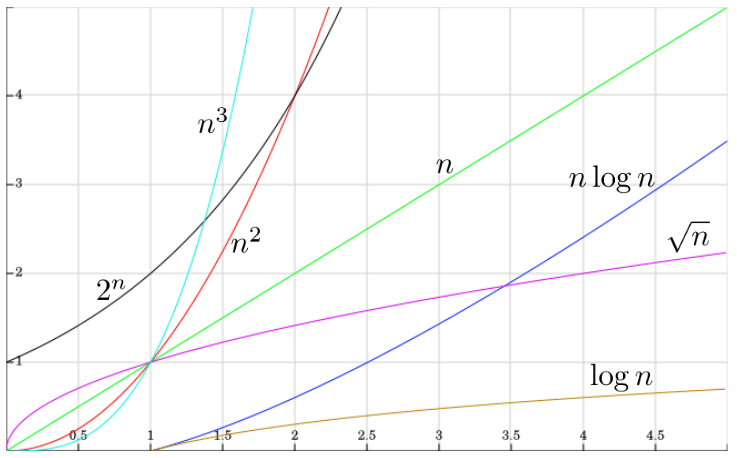
\includegraphics[scale=0.4]{img/runtime1.png}
\end{frame}

\begin{frame}[fragile]
\frametitle{Runtime Analysis}
Large input size\\
\centering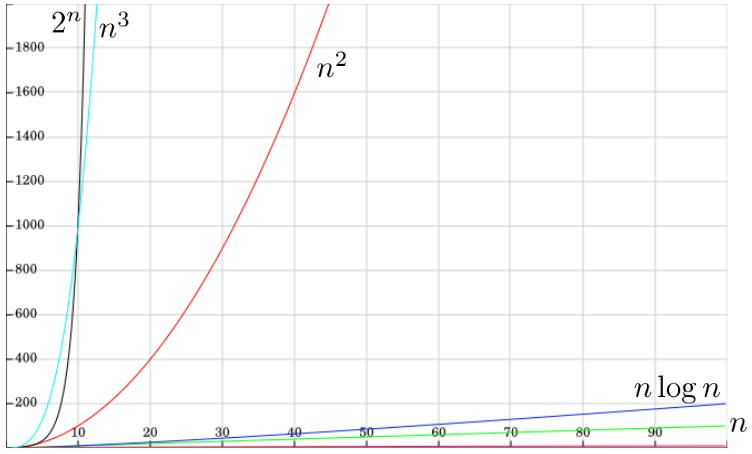
\includegraphics[scale=0.4]{img/runtime2.png}
\end{frame}

\begin{frame}[fragile]
\frametitle{Runtime Analysis}
\begin{example}
What is the runtime of \verb|method(n)|?
\begin{lstlisting}
void method(int n) {
  for (int i=0; i<n; i++) {
    for (int j=0; j<n; j++) {
      f();
    }
}
\end{lstlisting}
\end{example}

\end{frame}

\begin{frame}[fragile]
\frametitle{Runtime Analysis}
\begin{exercise}
Write a class \verb|RandomDataUtil| with a method\\
\verb|string createString(int size)| which creates a string, containing
random letters A-Z.\\
What is the runtime of your solution?
\end{exercise}

\end{frame}

\begin{frame}[fragile]
\frametitle{Runtime Analysis}
\begin{exercise}
Write a method, which takes a string (contains A-Z) as parameter. This method
should return the first character, which appears only one time
in this string.\\
What is the runtime of your solution?
\end{exercise}

\end{frame}


